\documentclass[10pt,a4paper]{article}
\usepackage[utf8]{inputenc}
\usepackage{amsmath}
\usepackage{amsfonts}
\usepackage{amssymb}
\usepackage{graphicx}
\usepackage[left=2cm,right=2cm,top=2cm,bottom=2cm]{geometry}
\usepackage{tikz}
\usepackage{subfiles}
\begin{document}

% \section*{Todo-list}

% \begin{itemize}
% \item Describe model
% \item Make example plots of model 
% \item Basic mathematical analysis of model
% \item Describe and illustrate isolines
% \item Show examples along isolines (both extremes and somewhere around middle)
% \item Make multiple simulations along particular isoline, and show relation between testProb and ratio of found recovered
% \item How to convert testProb to number of tests. Remember tests of S. Effect of testing previously recovered?
% \item Additional investigations: Different test-sensitivities (however, if test is 0.9 sens, then 1/0.9 tests should be made for same result)
% \item Check: How does testing of symptomatic change result?
% \end{itemize}


\section{Model-description}

The considered model is based on the classic SIR-model, 
extended to consider two stages of exposed prior to infectivity and a pre-symptomatic stage. 
Furthermore, asymptomatic individuals are considered, as well as individuals quarantined due to testing.
Symptomatic individuals are assumed to quarantine as well, and for simplicity, quarantine is asssumed to be perfect, i.e. quarantined individual do not contribute to the infectivity pressure.
Testing is assumed to be performed for all groups, excluding symptomatic cases. Only second stage of exposed, pre-symptomatic and asymptomatic are assumed to be found positive, and hence testing does not affect other groups. 
 
For purposes of analysis, we distinquish between recovered individuals that were quarantined due to testing and due to symptoms. However, we assume that all symptomatic cases get tested seperate from the testing considering within the model.

The full model formulation is given below:

\begin{align}
    \dot{S} &= - \beta S (P+A) \\ \label{eq:modeldefinition}
    \dot{E_1} &= \beta S (P+A) - \gamma E_1 \\
    \dot{E_2} &= \gamma E_1 - \gamma E_2 - \tau E_2\\
    \dot{P} &= \gamma E_2 - \gamma P - \tau P\\
    \dot{I} &= \gamma \rho P - \nu I \\
    \dot{A} &= \gamma (1-\rho) P - \nu A -\tau A \\
    \dot{Q} &= \tau (E_2 + P + A) - \nu Q \\
    \dot{R_p} &= \nu Q + \nu I \\
    \dot{R_n} &= \nu A 
\end{align}
Variables are scaled by population, such that $S+E_1+E_2+P+I+A+Q+R_p+R_n = 1$. 
Furthermore, one differential equation can in general be omitted as the full system sums to unity.

\begin{table}[h!] \centering
    \label{tab:modeldesc}\caption{}
\begin{tabular}{|r|l||r|l|}
    \hline 
    $S$ & susceptible & $E_1$, $E_2$ & Exposed \\
    $P$ & Pre-symptomatic & $I$ & Infectious (symptomatic, quarantined) \\
    $A$ & Asymptomatic & $Q$ & Quarantined (due to test) \\
    $R_p$ & Recovered, with positive test & $R_n$ & Recovered, no positive test \\
    \hline \hline 
    $\beta$ & Infecitivity & $\gamma $ & Rate of disease progression \\
    $\nu $ & Rate of recovery & $\rho $ & Fraction of symptomatic cases \\
    $ \tau $ & Rate of testing (effective) && \\
    \hline 
\end{tabular}
\end{table}

The total testing effort due to asymptomatic testing is given as $K_{\tau} = \tau (S+E_1 + E_2 + P + A + R_n)$. Note the contribution from $\tau R_n$. To account for the contribution of symptomatic testing, we consider the flow into the $I$ compartment, corresponding to immmediate testing when symptoms arise, $K_I = \gamma \rho P$. 
Total testing is given by $K_{tot} = K_{\tau} + K_I$. 

Note that $K_{\tau}(0) = \tau S$ and that $K_{\tau}  \underset{t \rightarrow \infty }{\longrightarrow} \tau (S+R_n)$. 

\section{Model analysis}
\subsection{Definitions and epidemic isolines}
The final size of an epidemic can be defined in terms of the proportion of the population that remains susceptible as time approaches infinity. 
We define $\sigma$ such that $S(t) \underset{t\rightarrow \infty}{\rightarrow} \sigma$. 
Similarly, the final size of the recovered population that were found positive through testing is defined as $R_p(t) \underset{t\rightarrow \infty}{\rightarrow} r_p$. 
Correspondingly, $R_n(t) \underset{t\rightarrow \infty}{\rightarrow} r_n$.  
We define the total recovered population, $r_{tot} = r_p + r_n$ and note that $r_{tot} + \sigma = 1$.
% Based on the intensity of testing, as given by parameter $\tau$, a proportion of the total recovered population $r_{tot}$

Figure \ref{fig:TestAndBeta} below, the bottom panel shows $r_{tot}$, as a function of model-parameters $\beta$ and $\tau$. 
In the top panel, $r_p$ is shown. Parts where $r_{tot} < 0.2$ are omitted in both plots.

\begin{figure}[h]\centering
    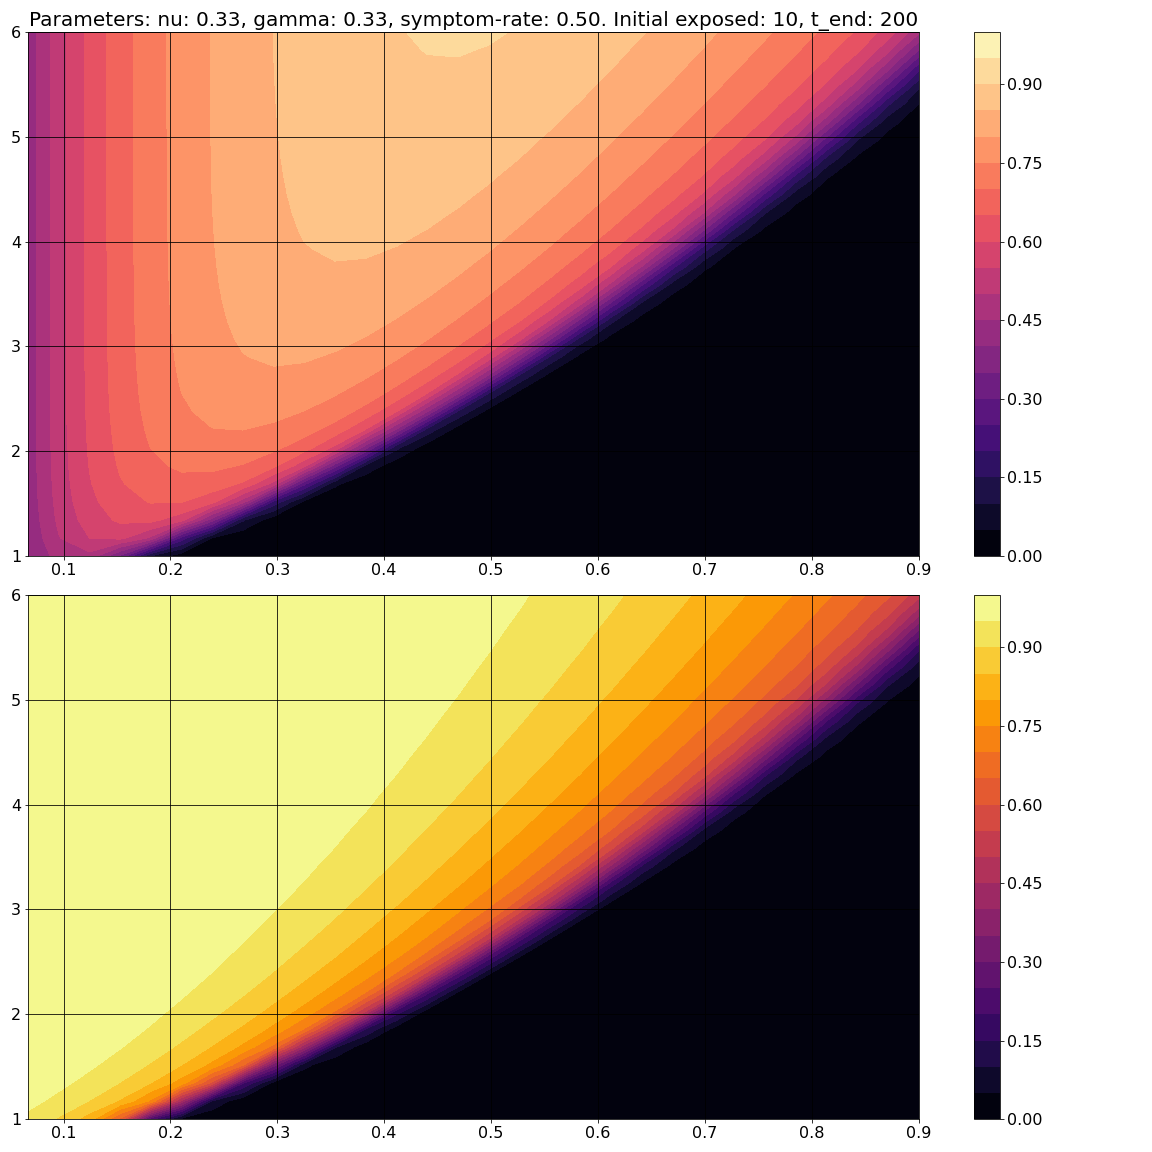
\includegraphics[width = \linewidth]{./../Figures/TestingModelling_TestProbAndInfectivity_Split.png}
    \caption{ }\label{fig:TestAndBeta}
\end{figure}

From the bottom panel of figure \ref{fig:TestAndBeta} we note that there exists combinations of $\beta$ and $\tau$ that yield the same final size of the epidemic. 
These exists along the contours given in the bottom panel of figure \ref{fig:TestAndBeta}.
This corresponds to the notion that testing effectively reduces the effective reproduction number. 
In the perspective of epidemic mitigation, this suggest that a disease with high infectivity (i.e. high $\beta$) requires a high level of testing to yield a final epidemic size comparable to a less infectious disease with lower levels of mitigation.
If $\beta$ describes the effective infectivity arising from different types of epicemic mitigation, the implication is that increased testing can make up a reduction in another unspecified part of the mitigation.
This model behaviour is expected and follows trivially from the model design of testing reducing infection pressure.
We refer to the lines of equal final size as epidemic isolines. 

While the final size is equal along an epidemic isoline, the number of infections identified by testing varies, as observed in the top panel of figure \ref{fig:TestAndBeta}.
We aim to investigate the relation between the intensity of testing, as given by parameter $\tau$, and the proportion of recovered individuals that were identified. 
We define the latter as $\theta = \frac{r_p}{r_{tot}}$. 
In figure \ref{fig:TestAndBetaComb} we show $\theta$ for the same range of $\beta$ and $\tau$ as in figure \ref{fig:TestAndBeta}.
The epidemic isolines are shown as red contourlines. Situations where $r_{tot} < 0.2$ are shown in grey for clarity.
\begin{figure}[h]\centering
    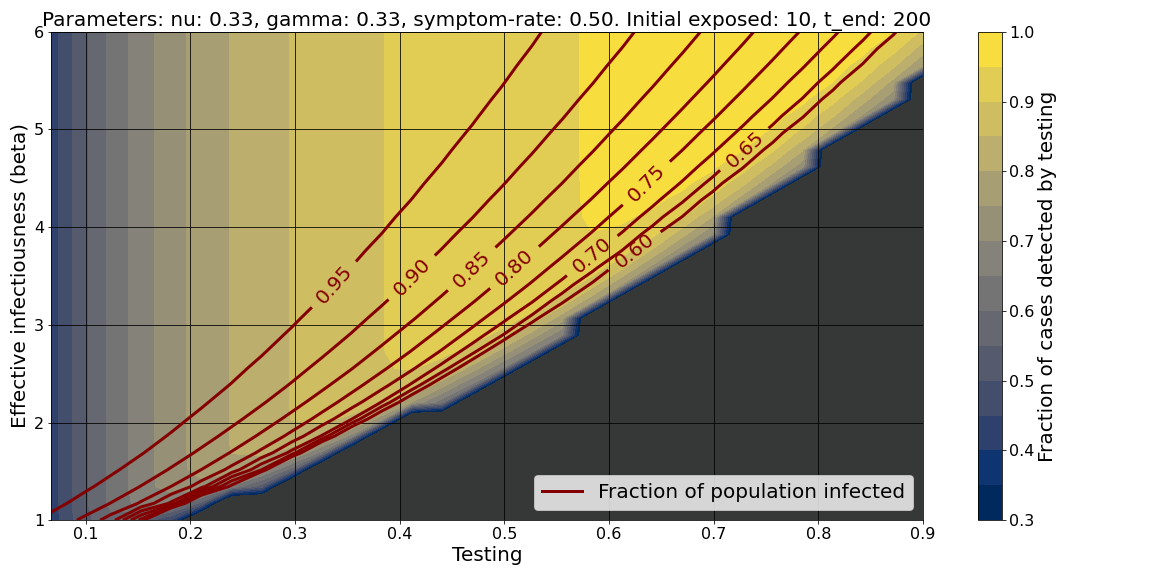
\includegraphics[width = \linewidth]{./../Figures/TestingModelling_TestProbAndInfectivity.png}
    \caption{Figure tex}\label{fig:TestAndBetaComb}
\end{figure}

\subsection{Characterization of epidemic isolines}
The relationship between a given testing intensity, $\tau$ and the infectiousness $\beta$ which yield final epicemic sizes along a epidemic isoline can be investigated analytically.
In practice, this allows for describing the isolines implicitly for a given final size.
In turn this allows us to describe the proportion of recovered infections that were identified for a given testing intensity, under the assumption that final epidemics size was unchanged.

Similar to the calculations of Andreasen (2018), we consider the following quantities based on the system of differential equations given in equations \eqref{eq:modeldefinition}

\begin{align}
    \dot{S} / S &= - \beta (P + A) \\
    \dot{S} + \dot{E_1} + \dot{E_2} &= -(\gamma + \tau) E_2 \\
    \dot{S} + \dot{E_1} + \dot{E_2} +\dot{P} &= -(\gamma + \tau) P - \tau E_2 \\
    \dot{S} + \dot{E_1} + \dot{E_2} + \dot{P} + \dot{A} &= -(\nu + \tau) A -(\gamma \rho + \tau) P - \tau E_2 
\end{align}

For simplicity, we assume that at time $t=0$, all variables except $S$ and $E_1$ are zero. 
As $t$ approaches infinity, the stability of the systems implies that all variables apart from $S$, $R_p$ and $R_n$ are zero. 

For notational purposes, we define for each variable $x$, the integral over the full epidemic as $T_x = \int_0^{\infty} x dt$.
Integrating the equations above over the entire epidemic yields:
\begin{align}
    \log{\sigma} &= - \beta (T_P - T_A) \\
    \sigma - S_0 - E_{1,0} &= - (\gamma + \tau) T_{E_2} \\
    \sigma - S_0 - E_{1,0} &= -(\gamma + \tau) T_P - \tau T_{E_2} \\
    \sigma - S_0 - E_{1,0} &= -(\nu + \tau) T_A -(\gamma \rho + \tau) T_P - \tau T_{E_2} 
\end{align}

Where $S_0$ and $E_{1,0}$ are initial conditions for $S(t)$ and $E_1(t)$ respectively. 
In the limit where $S_0 \rightarrow 1$ and $E_{1,0} \rightarrow 0$, we can rewrite:

\begin{align}
    \log{\sigma} &= - \beta (T_P - T_A) \\
    \sigma &= 1 - (\gamma + \tau) T_{E_2} \\
    \sigma &= 1 -(\gamma + \tau) T_P - \tau T_{E_2} \\
    \sigma &= 1 -(\nu + \tau) T_A -(\gamma \rho + \tau) T_P - \tau T_{E_2} 
\end{align}

Assuming $T_P + T_A \neq 0$, this can be written as:
\begin{align}
    \beta &= \dfrac{-\log \sigma}{T_P + T_A} \\
    T_{E_2} &= \frac{1}{\gamma + \tau} \left(1-\sigma \right)  \\
    T_P &= \frac{1}{\gamma + \tau}\left( 1 - \sigma - \tau T_{E_2} \right)\\
    T_A &= \frac{1}{\nu + \tau} \left(1 - \sigma -(\gamma \rho + \tau) T_P - \tau T_{E_2}\right)
\end{align}


Furthermore, observe that integrating $\dot{R_n} = \nu A$ from $t=0$ to $t=\infty$ yields $r_n = \nu T_A$. 

\subsection{Explicit expression for ratio of positive}
% 1 - (nu/(nu+tau))*(1-tau/(gamma+tau))*(1-(gamma*rho+tau)/(gamma+tau))
Combining the above equations reveal that 
\begin{align}
    \dfrac{r_p}{r_p+r_n} &= 1 - \dfrac{\nu}{1-\sigma} T_A \\
    \dfrac{r_p}{r_p+r_n} &= 1- \left(\dfrac{\nu}{\nu+ \tau} \right) \left(1- \dfrac{\tau}{\gamma+\tau} \right) \left(1-\dfrac{\gamma \rho + \tau}{\gamma + \tau}\right)
\end{align}
Note that this expression is independent of $\sigma$. 

Furthermore, in the absence of tests, i.e. for $\tau = 0$, the expression becomes $\dfrac{r_p}{r_p+r_n}  = 1- 1(1-0)(1-\rho) = \rho $. This is expected, as only the symptomatic cases, $I$, are found in the situation where $\tau=0$, and the symptomatic cases make up exactly $\rho$ of all cases.


\section{Numeric examples}
As an example, we consider $\nu = \gamma = \frac{1}{3}$ and $\rho = 0.5$. 
Setting $\sigma = 0.2$, and considering a range of $\tau$ between $0$ and $1$, we determine the corresponding values of $\beta$ using the equations above. 
The $(\tau,\beta)$-pairs give an epidemic isoline corresponding to $1-\sigma = 0.8$. This line is depicted in figure \ref{fig:IsolineExamples} below. 
In the figure, inset axes show time-series of $R_p(t)$ and $R_n(t)+R_p(t)$ obtained from numerical integration.

\begin{figure}[h]\centering
    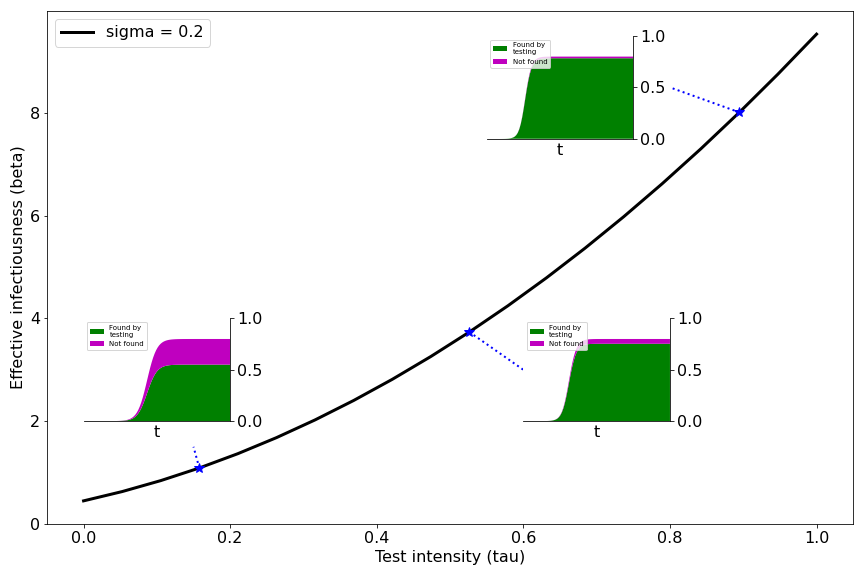
\includegraphics[width = \linewidth]{./../Figures/TestingModelling_IsolineExamples.png}
    \caption{ }\label{fig:IsolineExamples}
\end{figure}

We perform numerical integration for a range of $(\tau,\beta)$-pairs along the epidemic isoline. The resulting final values of $R_p(t)$ and $R_n(t)+R_p(t)$ are given in figure \ref{fig:AlongIsoline}.

\begin{figure}[h]\centering
    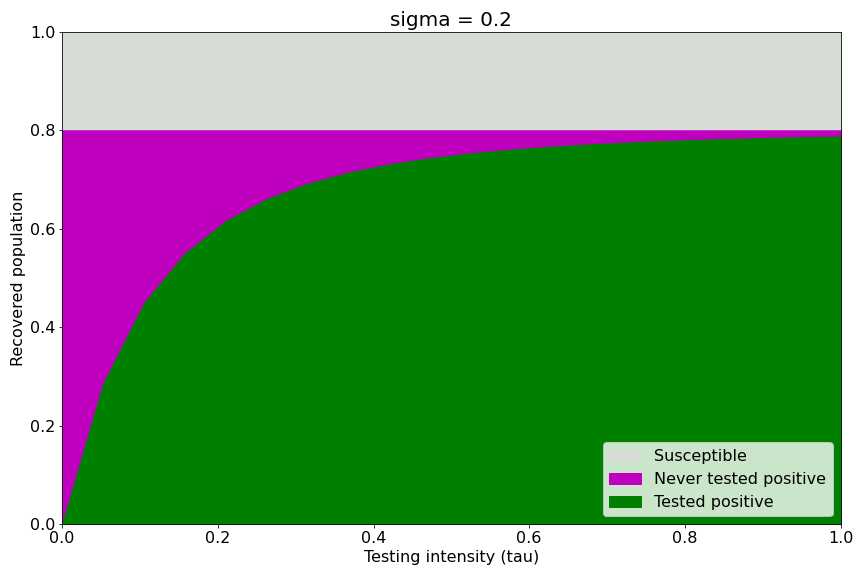
\includegraphics[width = \linewidth]{./../Figures/TestingModelling_AlongIsoline.png}
    \caption{ }\label{fig:AlongIsoline}
\end{figure}


\end{document}